\subsection{UC6 - Pausa trasferimenti}
\begin{figure}[H]
    \centering
    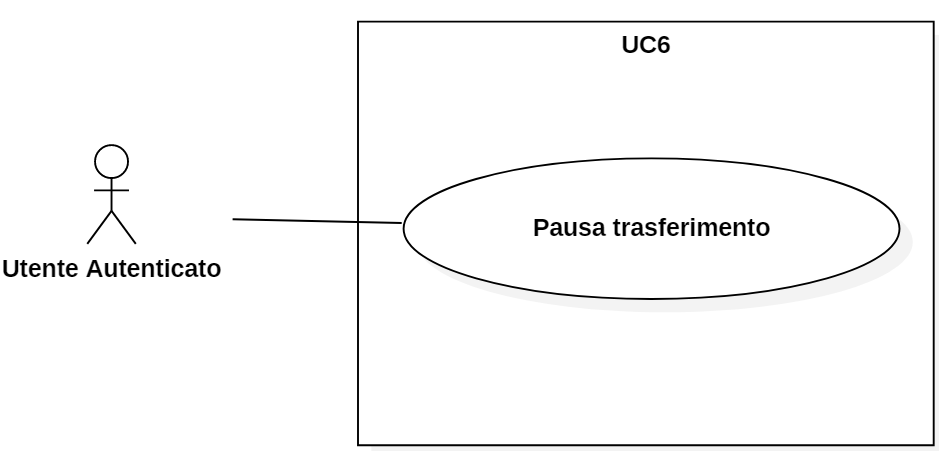
\includegraphics[scale = 0.4]{components/img/UC6.png}
    \caption{UC6 - Pausa trasferimenti}
\end{figure}
\begin{itemize}
\item \textbf{Attore Primario:} Utente autenticato;
\item \textbf{Precondizione:} L'utente ha a disposizione la possibilità di mettere in pausa il trasferimento di un file;
\item \textbf{Postcondizione:} Viene messo in pausa il trasferimento del file;
\item \textbf{Scenario principale:}
    \begin{enumerate}
    \item L'utente può mettere in pausa un file che si trova nello stato di trasferimento in corso.
    \end{enumerate}
\end{itemize}